\documentclass[a4paper,14pt,oneside,final]{extarticle}
\usepackage[top=2cm, bottom=2cm, left=3cm, right=1cm]{geometry}
\usepackage{scrextend}

\usepackage[T2A,T1]{fontenc}
\usepackage[ukrainian,russian,english]{babel}
\usepackage{tempora}
\usepackage{fontspec}
\setmainfont{tempora}

% Зачем: Отключает использование изменяемых межсловных пробелов.
% Почему: Так не принято делать в текстах на русском языке.
\frenchspacing

\usepackage{indentfirst}
\setlength{\parindent}{1.25cm}
\renewcommand{\baselinestretch}{1.5}

% Header
\usepackage{fancyhdr}
\pagestyle{fancy}
\fancyhead{}
\fancyfoot{}
\fancyhead[R]{\small \selectfont \thepage}
\renewcommand{\headrulewidth}{0pt}

% Captions
\usepackage{chngcntr}
\counterwithin{figure}{section}
\counterwithin{table}{section}
\usepackage[tableposition=top]{caption}
\usepackage{subcaption}
\DeclareCaptionLabelFormat{gostfigure}{Рисунок #2}
\DeclareCaptionLabelFormat{gosttable}{Таблиця #2}
\DeclareCaptionLabelSeparator{gost}{~---~}
\captionsetup{labelsep=gost}
\captionsetup[figure]{labelformat=gostfigure}
\captionsetup[table]{labelformat=gosttable}
\renewcommand{\thesubfigure}{\asbuk{subfigure}}

% Sections
\usepackage[explicit]{titlesec}
\newcommand{\sectionbreak}{\clearpage}

\titleformat{\section}
  {\centering}{\thesection \quad}{0pt}{\MakeUppercase{#1}}
\titleformat{\subsection}[block]
  {\bfseries}{\thesubsection \quad #1}{0cm}{}

\titlespacing{\section} {0cm}{0cm}{21pt}
\titlespacing{\subsection} {\parindent}{21pt}{0cm}
\titlespacing{\subsubsection} {\parindent}{0cm}{0cm}

% Lists
\usepackage{enumitem}
\renewcommand\labelitemi{--}
\setlist[itemize]{noitemsep, topsep=0pt, wide}
\setlist[enumerate]{noitemsep, topsep=0pt, wide, label=\arabic*}
\setlist[description]{labelsep=0pt, noitemsep, topsep=0pt, leftmargin=2\parindent, labelindent=\parindent, labelwidth=\parindent, font=\normalfont}

% Toc
\usepackage{tocloft}
\tocloftpagestyle{fancy}
\renewcommand{\cfttoctitlefont}{}
\setlength{\cftbeforesecskip}{0pt}
\renewcommand{\cftsecfont}{}
\renewcommand{\cftsecpagefont}{}
\renewcommand{\cftsecleader}{\cftdotfill{\cftdotsep}}

\usepackage{float}
\usepackage{pgfplots}
\usepackage{graphicx}
\usepackage{multirow}
\usepackage{amssymb,amsfonts,amsmath,amsthm}
\usepackage{csquotes}

\usepackage{listings}
\lstset{basicstyle=\footnotesize\ttfamily,breaklines=true}
\lstset{language=Matlab}

\usepackage[
	backend=biber,
	sorting=none,
	language=auto,
	autolang=other
]{biblatex}
\DeclareFieldFormat{labelnumberwidth}{#1}

\lstdefinelanguage{Python}{
  keywords={and, break, class, continue, def, yield, del, elif, else, except, exec, finally, for, from, global, if, import, in, lambda, not, or, pass, print, raise, return, try, while, assert, with},
  keywordstyle=\color{NavyBlue}\bfseries,
  ndkeywords={True, False},
  ndkeywordstyle=\color{BurntOrange}\bfseries,
  emph={as},
  emphstyle={\color{OrangeRed}},
  identifierstyle=\color{black},
  sensitive=true,
  commentstyle=\color{gray}\ttfamily,
  comment=[l]{\#},
  morecomment=[s]{/*}{*/},
  stringstyle=\color{ForestGreen}\ttfamily,
  morestring=[b]',
  morestring=[s]{"""*}{*"""},
}


\usepackage{tabularx}
\usepackage{multicol}

\newcommand{\labnumber}{3} % third lab
\documentclass[a4paper,14pt,oneside,final]{extarticle}
\usepackage[top=2cm, bottom=2cm, left=3cm, right=1cm]{geometry}
\usepackage{scrextend}

\usepackage[T2A,T1]{fontenc}
\usepackage[ukrainian,russian,english]{babel}
\usepackage{tempora}
\usepackage{fontspec}
\setmainfont{tempora}

% Зачем: Отключает использование изменяемых межсловных пробелов.
% Почему: Так не принято делать в текстах на русском языке.
\frenchspacing

\usepackage{indentfirst}
\setlength{\parindent}{1.25cm}
\renewcommand{\baselinestretch}{1.5}

% Header
\usepackage{fancyhdr}
\pagestyle{fancy}
\fancyhead{}
\fancyfoot{}
\fancyhead[R]{\small \selectfont \thepage}
\renewcommand{\headrulewidth}{0pt}

% Captions
\usepackage{chngcntr}
\counterwithin{figure}{section}
\counterwithin{table}{section}
\usepackage[tableposition=top]{caption}
\usepackage{subcaption}
\DeclareCaptionLabelFormat{gostfigure}{Рисунок #2}
\DeclareCaptionLabelFormat{gosttable}{Таблиця #2}
\DeclareCaptionLabelSeparator{gost}{~---~}
\captionsetup{labelsep=gost}
\captionsetup[figure]{labelformat=gostfigure}
\captionsetup[table]{labelformat=gosttable}
\renewcommand{\thesubfigure}{\asbuk{subfigure}}

% Sections
\usepackage[explicit]{titlesec}
\newcommand{\sectionbreak}{\clearpage}

\titleformat{\section}
  {\centering}{\thesection \quad}{0pt}{\MakeUppercase{#1}}
\titleformat{\subsection}[block]
  {\bfseries}{\thesubsection \quad #1}{0cm}{}

\titlespacing{\section} {0cm}{0cm}{21pt}
\titlespacing{\subsection} {\parindent}{21pt}{0cm}
\titlespacing{\subsubsection} {\parindent}{0cm}{0cm}

% Lists
\usepackage{enumitem}
\renewcommand\labelitemi{--}
\setlist[itemize]{noitemsep, topsep=0pt, wide}
\setlist[enumerate]{noitemsep, topsep=0pt, wide, label=\arabic*}
\setlist[description]{labelsep=0pt, noitemsep, topsep=0pt, leftmargin=2\parindent, labelindent=\parindent, labelwidth=\parindent, font=\normalfont}

% Toc
\usepackage{tocloft}
\tocloftpagestyle{fancy}
\renewcommand{\cfttoctitlefont}{}
\setlength{\cftbeforesecskip}{0pt}
\renewcommand{\cftsecfont}{}
\renewcommand{\cftsecpagefont}{}
\renewcommand{\cftsecleader}{\cftdotfill{\cftdotsep}}

\newcommand{\khpistudentgroup}{КН-34г}
\newcommand{\khpistudentname}{Чепурний~А.~С.}

\newcommand{\khpidepartment}{Програмна інженерія та інформаційні технології управління}
\newcommand{\khpititlewhat}{
	Лабораторна робота №\labnumber \\
	з предмету <<Моделювання систем>>
}
\newcommand{\khpititlewho}{
	Виконав: \\
	\hspace*{\parindent} ст. групи \khpistudentgroup \\
	\hspace*{\parindent} \khpistudentname \\
	Перевірила: \\
	\hspace*{\parindent} ст. в. каф. ПІІТУ \\
	\hspace*{\parindent} Єршова~С.~І. \\
	\hspace*{\parindent} ас. каф. ПІІТУ \\
	\hspace*{\parindent} Литвинова~Ю.~С. \\
}



\graphicspath{{figures/}}

\begin{document}
\Ukrainian

\begin{titlepage}

\begin{center}
	МІНІСТЕРСТВО ОСВІТИ І НАУКИ УКРАЇНИ \\
	НАЦІОНАЛЬНИЙ ТЕХНІЧНИЙ УНІВЕРСИТЕТ \\
	«ХАРКІВСЬКИЙ ПОЛІТЕХНІЧНИЙ ІНСТИТУТ» \\[0.5cm]
	Кафедра <<\khpidepartment>> \\
\end{center}

\vspace{6cm}

\begin{center}
	\khpititlewhat
\end{center}

\vspace{3cm}

\begin{addmargin}[10cm]{0cm}
	\khpititlewho
\end{addmargin}

\vspace{\fill}

\begin{center}
	Харків \the\year
\end{center}

\end{titlepage}

\addtocounter{page}{1}

\section{Основы YARN}
\subsection*{Цель}
Исследование пакетного менеджера YARN.
\subsection*{Задачи}
\begin{itemize}
    \item выявить преимущества и недостатки YARN;
    \item проанализировать этапы создания YARN-приложения;
    \item проанализировать разные модели программирования YARN.
\end{itemize}

\subsection{Менеджер управления ресурсами YARN}
YARN (англ.  Yet Another Resource Negotiator --- <<ещё один ресурсный посредник>>) --- модуль, отвечающий за управление ресурсами кластеров и планирование заданий. 
YARN функционирует как самостоятельный демон -- планировщик ресурсов, абстрагирующий все вычислительные ресурсы кластера и управляющий их предоставлением приложениям распределённой обработки. 
Под управлением YARN могут работать как MapReduce-программы, так и любые другие распределённые приложения, поддерживающие соответствующие программные интерфейсы. YARN обеспечивает возможность параллельного выполнения нескольких различных задач в рамках кластера и их изоляцию по принципам мультиарендности. 

Ключевые компоненты:
\begin{itemize}
    \item ResourceManager (RM) --- менеджер ресурсов, задачей которого является распределение ресурсов, необходимых для работы приложений, и наблюдение за вычислительными узлами, на которых эти приложения выполняются.
    \item ApplicationMaster (AM) --- компонент, ответственный за планирование жизненного цикла, координацию и отслеживание статуса выполнения распределенного приложения. Каждое приложение имеет свой экземпляр ApplicationMaster. ApplicationMaster управляет всеми аспектами жизненного цикла, включая динамическое увеличение и уменьшение потребления ресурсов, управление потоком выполнения, обработку ошибок и искажений вычислений и выполнение других локальных оптимизаций. Фактически, AM может выполнять произвольный пользовательский код и может быть написан на любом языке программирования, поскольку вся связь с RM и NM кодируется с использованием расширяемых протоколов связи.
    \item NodeManager (NM) --- агент, запущенный на вычислительном узле и отвечающий за отслеживание используемых вычислительных ресурсов (ЦП, RAM и т.д.), за управление логами и за отправку отчетов по используемым ресурсам планировщику менеджера ресурсов ResourceManager/Scheduler. NodeManager управляет абстрактными контейнерами, которые представляют собой ресурсы на узле, доступные для конкретного приложения.
    \item Контейнер (Container) --- набор физических ресурсов, таких как ЦП, RAM, диски и др. в одной ноде.
\end{itemize}

\subsection{Недостатки MRv1}
У первой версии MapReduce были как сильные, так и слабые стороны. MRv1 является стандартом системы обработки больших данных. 
Тем не менее эта архитектура имеет недостатки, которые в основном проявляются в больших кластерах. Если число узлов в кластере превышает 4000 (каждый узел может быть многоядерным), возникает некоторая непредсказуемость. Одна из самых больших проблем --- каскадные сбои, когда точечный сбой приводит к серьезному повреждению всего кластера из-за попыток репликации данных и перегрузки работоспособных узлов (вследствие <<затопления>> сети сообщениями).

Но самой большой проблемой MRv1 является совместная аренда. По мере того как размер кластеров растет, возникает желание использовать их для разных моделей применения. MRv1 выделяет для Hadoop узлы, которые можно перенацеливать на другие приложения и рабочие нагрузки. Растущая роль больших данных и Hadoop в облачных средах ведет к углублению этой тенденции, поскольку такая модель использования делает возможной локализацию Hadoop на физических серверах с отказом от виртуализации и связанных с ней добавочных издержек управления, вычисления и ввода/вывода.

\subsection{Введение в YARN (MRv2)}
Чтобы улучшить совместное использование, масштабируемость и надежность кластера Hadoop, был выбран иерархический подход к инфраструктуре кластера. В частности, узкоспециализированная функциональность MapReduce была заменена новым набором демонов, который открывает инфраструктуру для новых моделей обработки.

Подход с использованием JobTracker и TaskTracker был главным недостатком MRv1 из-за ограничений масштабирования и наличия режимов отказов, вызванных сетевыми издержками. Эти демоны были также характерны для модели обработки MapReduce. С целью ликвидировать эту зависимость JobTracker и TaskTracker были удалены из YARN и заменены новым набором демонов, не привязанных к приложениям.

Новая архитектура YARN представлена на рисунке~\ref{fig:yarn_arch}.

\begin{figure}[H]
    \centering
    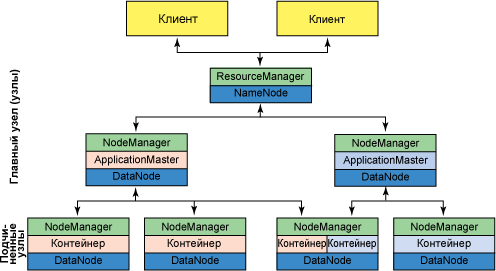
\includegraphics[width=0.8\textwidth]{yarn_arch}
    \caption{Новая архитектура YARN}
    \label{fig:yarn_arch}
\end{figure}

С приходом YARN исчезли ограничения парадигмы разработки, присущие прежней модели MapReduce, и появилась возможность создания более сложных распределенных приложений. Фактически модель MapReduce --- это лишь одно приложение в наборе, который может выполнять архитектура YARN, которая выходит за рамки базовой инфраструктуры для специализированной разработки. Сила YARN в том, что ее использование потенциально безгранично и больше не требует (в отличие от MRv1) изоляции от других, более сложных распределенных интегрированных сред, работающих на кластере. По мере того как YARN будет становиться надежнее, она сможет заменить некоторые другие инфраструктуры распределенной обработки, полностью высвободив выделенные им ресурсы, а также упростив систему в целом.

Для иллюстрации эффективности YARN в сравнении с MRv1 рассмотрим параллельную задачу расшифровки путем полного перебора хеша LAN Manager, который раньше использовался в Windows® для хеширования паролей. В этом случае методика MapReduce не имеет смысла из-за слишком высоких издержек на этапах отображения/сокращения. Более логичным является распределение нагрузки, при котором каждый контейнер получает часть области поиска, выполняет перебор и сообщает о нахождении правильного пароля. Идея в том, чтобы определять пароль динамически с помощью функции (побитовой обработки) вместо отображения всех возможных вариантов в структуру данных, которое делает стиль MapReduce избыточным и громоздким.

\subsection{Запуск приложения в YARN}
В этом разделе описывается взаимодействие процессов ResourceManager, ApplicationMaster, NodeManager и контейнеров при запуске приложения в кластере YARN.

Запуск приложения в YARN представлен на рисунке~\ref{fig:yarn_sample}.

\begin{figure}[H]
    \centering
    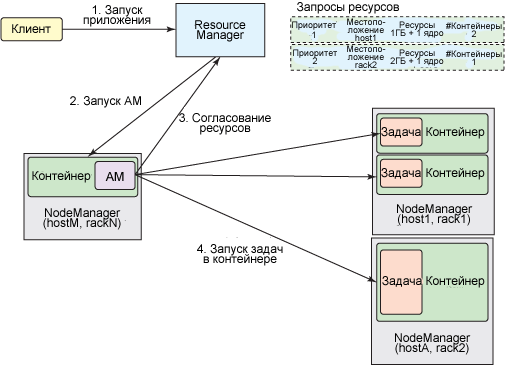
\includegraphics[width=0.8\textwidth]{yarn_sample}
    \caption{Запуск приложения в YARN}
    \label{fig:yarn_sample}
\end{figure}

Пользователи запускают приложения в ResourceManager с помощью команды \texttt{hadoop jar} по аналогии с MRv1. ResourceManager обрабатывает список выполняющихся в кластере приложений и список доступных ресурсов в каждом работоспособном NodeManager. ResourceManager должен определить приложение для получения следующей порции ресурсов кластера. На это решение влияет много ограничений, например вместимость очереди, списки управления доступом и равнодоступность ресурсов. ResourceManager использует подключаемый планировщие (Scheduler). Scheduler занимается только планированием, определяя очередность получения ресурсов кластера (в виде контейнеров), но не выполняет мониторинг задач в приложении и не пытается перезапустить задачи после сбоев.

Когда ResourceManager подтверждает запуск нового приложения, одним из первых решений Scheduler является выбор контейнера, в котором будет выполняться ApplicationMaster. Запущенный ApplicationMaster отвечает за весь жизненный цикл данного приложения. В первую очередь это будет передача в ResourceManager запроса ресурсов в виде контейнеров для выполнения задач приложения. Запрос ресурсов -- это просто запрос числа контейнеров, удовлетворяющих следующим требованиям к ресурсам:

Объем ресурсов --- память в мегабайтах и доля вычислительных ресурсов процессора.
Предпочитаемое местоположение --- имя хоста (hostname), имя стойки (rackname) или * при отсутствии предпочтений.
Приоритет в этом приложении, а не в нескольких приложениях.
Если (и когда) это возможно, ResourceManager предоставляет контейнер (описываемый идентификатором контейнера и именем хоста), который удовлетворяет требованиям, содержащимся в запросе ресурсов. Контейнер позволяет приложению использовать указанный объем ресурсов на конкретном хосте. После предоставления контейнера ApplicationMaster дает команду NodeManager (который управляет хостом, где был размещен контейнер) использовать эти ресурсы для запуска задачи данного приложения. Этой задачей может быть любой процесс, созданный в любой инфраструктуре (например, задача MapReduce или задача Giraph). NodeManager не отслеживает задачи; он лишь выполнят мониторинг использования ресурсов в контейнере, например, для удаления контейнера, потребляющего больше памяти, чем ему было выделено.

ApplicationMaster тратит все свое время на согласование контейнеров для запуска задач приложения. Он также следит за выполнением приложения и его задач, перезапускает задачи после сбоев в созданных контейнерах и предоставляет отчеты о выполнении клиенту, запустившему приложение. После завершения приложения ApplicationMaster выключается и освобождает свой собственный контейнер.

Хотя ResourceManager не выполняет мониторинг задач приложения, он проверяет состояние процессов ApplicationMaster. В случае сбоев ResourceManager может перезапустить ApplicationMaster в новом контейнере. Можно сказать, что ResourceManager заботится об ApplicationMaster, а ApplicationMaster заботится о задачах.

\subsection*{Выводы}
Менеджер управления ресурсами YARN является улучшением системы MRv1 и позволяет обойти много ее проблем, таких как:
\begin{itemize}
    \item каскадные сбои, когда точечный сбой приводит к серьезному повреждению всего кластера из-за попыток репликации данных и перегрузки работоспособных узлов (вследствие <<затопления>> сети сообщениями);
    \item совместная аренда. 
\end{itemize}

\end{document}
